\subsection{Conjunto de datos}
\begin{figure}[H]
    \centering
    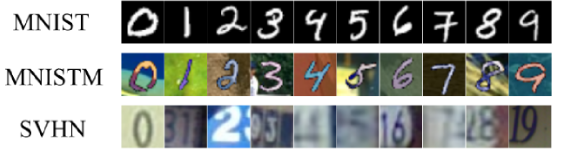
\includegraphics[width=\linewidth]{../images/domains.png}
    \caption{Ejemplos de dígitos de los tres dominios que se utilizaron}
    \label{fig:domain}
\end{figure}

Como se puede observar en la imagen~\ref{fig:domain} se trabajó con tres conjuntos de datos de dígitos (0-9) que presentan diferencias visuales importantes entre sí. MNIST es un conjunto de 70000 digitos escritos a mano en escala de grises, MNIST-M son 59.000 digitos sobre fondos fotográficos a color y SVHN presenta 99.289 dígitos en imágenes de casas reales. Los tres datasets fueron divididos en train, validation y test.

Dado que los conjuntos no comparten el mismo formato de imagen, fue necesario aplicar una etapa de preprocesamiento antes del entrenamiento. En particular, se unificó el tamaño de todas las imágenes a 32×32 píxeles y se llevó la cantidad de canales a tres. Esto implicó convertir las imágenes de MNIST, originalmente en escala de grises, a una representación RGB de tres canales, para que tuvieran la misma dimensionalidad que MNIST-M y SVHN. Además, las imágenes fueron normalizadas utilizando la media y el desvío estándar correspondientes a cada dataset. Este procedimiento permitió que todos los modelos recibieran entradas con la misma forma.

\subsection{Entrenamiento episódico y configuración few-shot}
Para entrenar los modelos de meta-learning se puede utilizar un esquema de muestreo episódico. A diferencia del entrenamiento supervisado tradicional, donde el modelo aprende a partir de batches formados aleatoriamente sobre todo el conjunto de datos, en el entrenamiento episódico cada batch simula una pequeña tarea de clasificación few-shot. De esta manera, el modelo no aprende solamente a clasificar un conjunto fijo de clases, sino a adaptarse a tareas nuevas construidas con pocos ejemplos.

Cada episodio se define mediante tres parámetros principales: $N$, $K$ y $Q$. El valor $N$ indica la cantidad de clases muestreadas en ese episodio. El valor $K$ indica la cantidad de ejemplos etiquetados disponibles por clase en el conjunto de soporte (\textit{support set}). Finalmente, $Q$ indica la cantidad de ejemplos de consulta por clase, es decir, las imágenes del \textit{query set} sobre las cuales se evalúa el desempeño del modelo dentro del episodio. Los parámetros se presentan como ``$N$-way, $K$-shot, $Q$=q".

\subsection{Prototypical Networks}
Las \textit{Prototypical Networks} (ProtoNets), propuestas por \textit{Snell et al.} (2017)\footnote{\url{https://arxiv.org/abs/1703.05175}}, son un método de meta learning diseñado para tareas de clasificación few-shot. La idea principal consiste en aprender un espacio de embeddings donde ejemplos pertenecientes a una misma clase se agrupen bien.

Durante cada episodio de entrenamiento, el modelo recibe un conjunto de soporte y un conjunto de consulta. Para cada clase $n$, se calcula un ``prototipo'' como el promedio de los embeddings de las muestras de soporte:

\begin{equation}
c_n = \frac{1}{K}
\sum_{\substack{(x,y)\in D^{\text{tr}} \\ y=n}}
f_\theta(x),
\end{equation}

donde $f_\theta(x)$ es el embedding resultante de la red $f_\theta$ para la muestra $x$, $K$ es el número de muestras de soporte por clase, y $D^{\text{tr}}$ es el conjunto de soporte.

Luego, la probabilidad de que una imagen de query $x$ pertenezca a la clase $n$ es:

\begin{equation}
p_\theta(y=n|x) =
\frac{
\exp\left(-\|\left(f_\theta(x)-c_n\right)\|^2\right)
}{
\sum_{n'} \exp\left(-\|\left(f_\theta(x)-c_{n'}\right)\|^2\right)
}.
\end{equation}

La actualización de pesos utiliza la métrica de entropía cruzada sobre esa probabilidad.

\subsection{MAML}
\textit{Model-Agnostic Meta-Learning} (MAML), propuesto por \textit{Finn et al.} (2017)\footnote{\url{https://arxiv.org/abs/1703.03400}}, es otro enfoque cuyo objetivo es aprender una inicialización de parámetros capaz de adaptarse rápidamente a nuevas tareas mediante unas pocas iteraciones de descenso por gradiente.

Durante cada episodio, el modelo realiza una adaptación interna utilizando el conjunto de soporte:

\begin{equation}
\theta'_i = \theta - \alpha \nabla_\theta
\mathcal{L}_{\mathcal{T}_i}^{support}(\theta),
\end{equation}

con $\alpha$ el learning rate y $\theta'_i$ los parámetros adaptados para la tarea $\mathcal{T}_i$.

Posteriormente en el \textit{outer loop} se evalúa el desempeño sobre el conjunto de consulta y se optimizan los parámetros originales minimizando:

\begin{equation}
\min_\theta \sum_{\mathcal{T}_i}
\mathcal{L}_{\mathcal{T}_i}^{query}(\theta'_i).
\end{equation}

Al minimizar por gradiente descendiente, se necesitan calcular gradientes de segundo orden.

A diferencia de métodos basados en métricas, MAML aprende explícitamente cómo adaptarse mediante gradientes, permitiendo una rápida especialización a nuevas tareas. Sin embargo, el entrenamiento puede resultar inestable y computacionalmente costoso debido al cálculo de gradientes de segundo orden.

\subsection{ProtoMAML}

ProtoMAML, propuesto por \textit{Triantafillou et al.} (2020)\footnote{\url{https://arxiv.org/abs/1903.03096}}, combina ideas de Prototypical Networks y MAML. El objetivo es aprovechar la estabilidad de los métodos métricos junto con la capacidad de adaptación rápida basada en optimización.

En ProtoMAML, los prototipos calculados a partir del conjunto de soporte se utilizan para inicializar dinámicamente la capa clasificadora antes de realizar las actualizaciones internas de MAML. Dados los prototipos $\mathbf{p}_c$, los pesos y sesgos del clasificador se inicializan como:

\begin{equation}
w_c = 2p^{\intercal}_c,
\end{equation}

\begin{equation}
b_c = -\|p_c\|^2.
\end{equation}

Este método, en teoría, produce predicciones equivalentes a las Prototypical Networks. Luego, a partir de este punto de partida, los pasos de adaptación refinan los parámetros logrando converger en considerablemente menos pasos que una inicialización aleatoria.

\subsection{DANN}

La \textit{Domain-Adversarial Neural Network} (DANN), propuesta por \textit{Ganin et al.} (2016)\footnote{\url{https://arxiv.org/abs/1505.07818}}, es un método de domain adaptation cuyo objetivo es aprender representaciones invariantes al dominio.

La arquitectura consta de tres componentes principales: un extractor de características, un clasificador de etiquetas y un clasificador de dominio.

El extractor de características se entrena para minimizar simultáneamente el error de clasificación y maximizar el error del clasificador de dominio. Esto se logra mediante una capa denominada \textit{Gradient Reversal Layer} (GRL), que invierte el signo del gradiente durante la retropropagación.

La función objetivo puede expresarse como:

\begin{equation}
\mathcal{L}_{DANN} =
\mathcal{L}_{task} - \lambda \mathcal{L}_{domain},
\end{equation}

donde $\mathcal{L}_{task}$ corresponde a la pérdida de clasificación principal y $\mathcal{L}_{domain}$ a la pérdida del discriminador de dominio. El valor de $\lambda$ aumenta a lo largo del entrenamiento para que el encoder pueda construir buenos features iniciales con menor intervención de $\mathcal{L}_{domain}$.

\begin{equation}
    \lambda_p = \frac{2}{1 + e^{-10p}} - 1, \qquad p \in [0, 1]
\end{equation}

De esta manera, el modelo aprende a clasificar y a confundir al discriminador simultáneamente, generando embeddings útiles pero indistinguibles entre dominios fuente y objetivo. Esto favorece la generalización ante un \textit{domain shift}.